\documentclass{article}
\usepackage{graphicx} % Required for inserting images

\begin{document}
\section{CapstoneVisionSegmentation: Room Segmentation Method Based on Computer Vision}
\subsection{Method Overview}
CapstoneVisionSegmentation is a rule-based method designed to segment interior spaces from architectural floor plans provided in GeoJSON format. Unlike supervised deep learning approaches, this method leverages classical computer vision techniques to extract room boundaries from geometric data, without requiring training datasets.

The pipeline consists of converting vector data into raster images, applying image processing operations to detect closed areas, and exporting the resulting room contours back into a georeferenced vector format (GeoJSON). The entire workflow is based on OpenCV image processing primitives and geospatial data transformations.

\subsection{Pipeline Description}

The method is structured in the following key steps:

\begin{enumerate}
    \item \textbf{Vector Preprocessing.} 
    Raw GeoJSON data often includes heterogeneous geometries (Polygons, MultiPolygons, LineStrings), many of which are noisy or incomplete. We filter the data to retain only the linear primitives representing walls. The geometries are rescaled and recentered to ensure consistent metric resolution before conversion.

    \item \textbf{Binary Image Generation.} 
    The preprocessed segments are rasterized into binary black-and-white images, where each segment is drawn with a configurable thickness (default: 3 pixels). A DPI value of 50 (50 pixels per meter) ensures sufficient spatial resolution. To improve the connectivity of wall segments, we apply Gaussian dilation, which smooths the edges and ensures continuity even in curved or oblique wall segments.

    \begin{figure}[h]
        \centering
        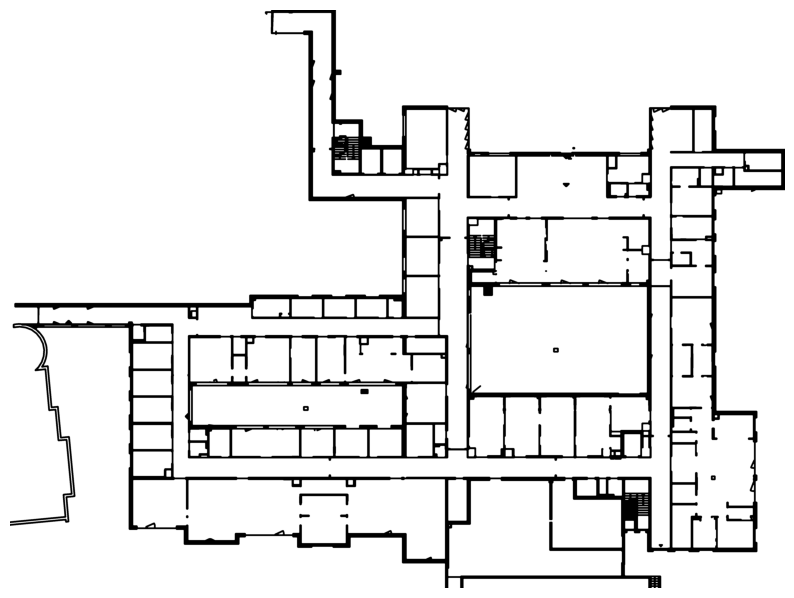
\includegraphics[width=0.6\linewidth, height=4cm, keepaspectratio]{01.binary_image.png}
        \caption{Example of a binary image generated from vector segments.}
        \label{fig:binary_image}
    \end{figure}

    \item \textbf{Morphological Processing and Contour Detection.} 
    A morphological closing operation (cv2.morphologyEx with MORPH\_CLOSE) fills small gaps between wall segments. Contours are then extracted with cv2.findContours using the RETR\_CCOMP mode, producing a hierarchical tree structure that allows holes (e.g., internal courtyards or voids) to be identified and processed correctly.

    \item \textbf{Wall Filtering and Room Selection.} 
    To discriminate between rooms and walls, we apply geometric criteria. Only contours with a surface area greater than 1 m² (2500 pixels at 50 DPI) and an average thickness (surface-to-perimeter ratio) exceeding 0.4 meters are retained. Additionally, the longest contour—typically representing the building envelope—is discarded.

    \item \textbf{Polygon Conversion and GeoJSON Export.} 
    The valid contours are converted back into metric coordinates using transformation parameters from the rasterization step. Polygons are enriched with properties such as area (m²) and a unique room identifier. Final outputs are exported in GeoJSON format for use in spatial analysis or digital twin generation.
    
    \begin{figure}[h]
        \centering
        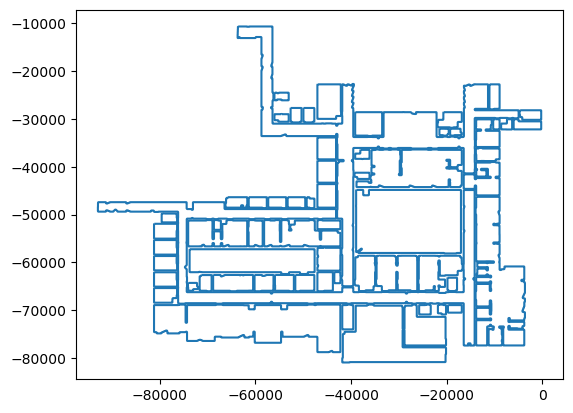
\includegraphics[width=0.48\linewidth]{04.rooms_contours_geojson.png}
        \hfill
        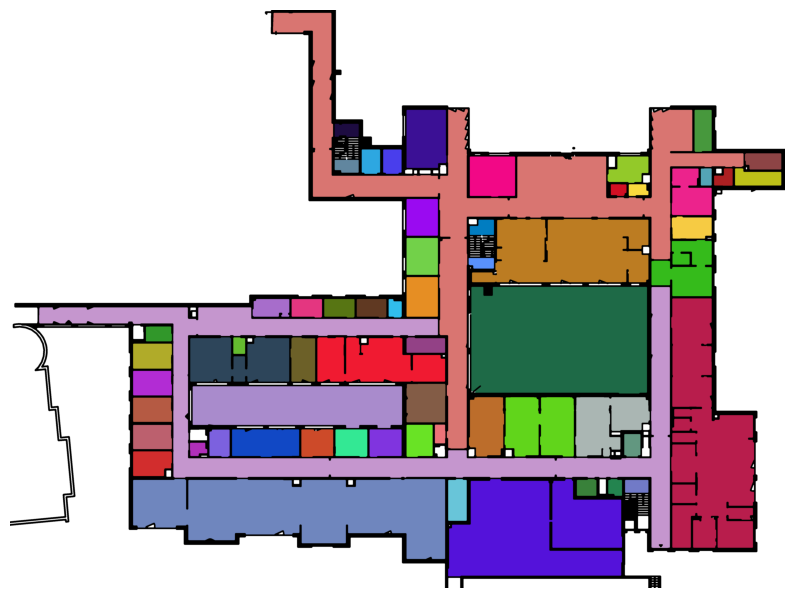
\includegraphics[width=0.48\linewidth]{02.contours_image.png}
        \caption{Left: GeoJSON export of room contours. Right: Colorized visualization of detected rooms.}
        \label{fig:geojson_and_colored}
    \end{figure}

\end{enumerate}

\subsection{Model Parameters}

\begin{table}[h]
    \centering
    \begin{tabular}{|l|l|}
        \hline
        \textbf{DPI}: & 50 pixels per meter (1 pixel $\approx$ 2 cm) \\ \hline
        \textbf{Wall thickness}: & 3 pixels (default) \\ \hline
        \textbf{Minimum room area}: & 1 m² \\ \hline
        \textbf{Minimum average thickness}: & 0.4 m \\ \hline
        \textbf{Dilation method}: & Gaussian \\ \hline
    \end{tabular}
    \caption{Model Parameters}
    \label{tab:model_checkpoint}
\end{table}

\subsection{Discussion}

CapstoneVisionSegmentation offers a simple yet robust solution for room segmentation on vector floor plans. It avoids the complexity of enforcing strict topological rules in vector space and instead leverages the flexibility of raster-based computer vision techniques. The method is particularly suited to noisy, incomplete, or low-quality CAD/BIM exports where traditional vector-based approaches fail.

However, the method depends on the explicit representation of physical separations. In cases where doors are missing or open connections are not physically modeled, adjacent spaces may be incorrectly merged into a single room.

\end{document}
